\documentclass{homework}
\usepackage[utf8]{inputenc}
\usepackage{xspace,color,url,listings,graphicx,float,amsmath,amssymb,braket,subcaption}
\graphicspath{{./graphs/}} %location of images

\lstset{commentstyle=\color{red},keywordstyle=\color{black},
showstringspaces=false}
\lstnewenvironment{rc}[1][]{\lstset{language=Python}}{}
\newcommand{\ri}[1]{\lstinline{#1}}  %% Short for 'R inline'

\lstset{language=Python}             % Set Py to default language

\newcommand{\hwname}{Shara Duong, Charles Colgan, Josh Borders}
\newcommand{\hwnum}{1}

\newcommand{\hwtype}{Homework}
\newcommand{\hwclass}{MATH 6373}

\begin{document}

\maketitle

Shara Duong: Wrote and edited code\\
Charles Colgan: Edited report\\
Josh Borders: Wrote the report.

\question*{Introduction and Data Description}
Our goal is to implement a Multi-Layer Perceptron (MLP) to predict the price of the American Dollar (USD) with respect to the Japanese Yen (JPY). To do so, we utilized the historic value of the Yen along with three other financial metrics as correlated features: Canadian Dollars (CAD), Mexican Pesos (MXN), and the S\&P 500 index (SP). CAD and MXN are positively related to the price of the dollar in yen as all three countries are popular trading partners with the United States. SP is used as a proxy for the underlying strength of USD. \\\\ 
We collected 1231 trading days of data quoted via investing.com, from February 8, 2016 to January 29, 2021. Below is the oldest observation, from 02-08-2016:\\\\
\begin{pmatrix}
CAD&MXN&JPY&SP&CAD(t-1)&MXN(t-1)&...&JPY(t-3)&SP(t-3)&\textbf{JPY(t+1)}\\
1.39&18.65&116.95&1853.44&1.38&18.45&...&119.85&1912.53&\textbf{115.67}
\end{pmatrix}\\\\
where CAD is the value of Canadian Dollars in USD, MXN is the value of Mexican Pesos in USD, JPY is the number of yen required, and SP is the value of the S&P500 index. (t-i) indicates the recorded value of the metric i days prior. JPY(t+1), also referred to as Y(t), is the response variable which the MLP is attempting to predict. The MLP's input is a row vector, V(t), of dimension 16, containing the recorded value of each metric for a given day and the 3 days prior. The output, MLP[JPY(t+1)], is the predicted value of yen in USD.\\\\
A heatmap displaying the correlation coefficients between the features and Y(t), which is equivalent to JPY(t+1), is provided in Figure \ref{corr}. Unsurprisingly, the features are highly correlated with their values from the previous days, taking values close to one. The rest of the correlations are relatively weak though, with the MXN and CAD carrying the strongest value at around 0.6. The bottom row of Figure \ref{corr} displays the correlations between the output variable, Y(t), and the features. Apart from previous values of JPY, Y(t) has very weak, slightly negative correlations with the rest of the chosen indices.\\\\
The series of Y(t) is displayed in Figure \ref{yt}. All of the indices, after normalization, are displayed in Figure \ref{allseries}.

\begin{figure}[h]
    \centering
    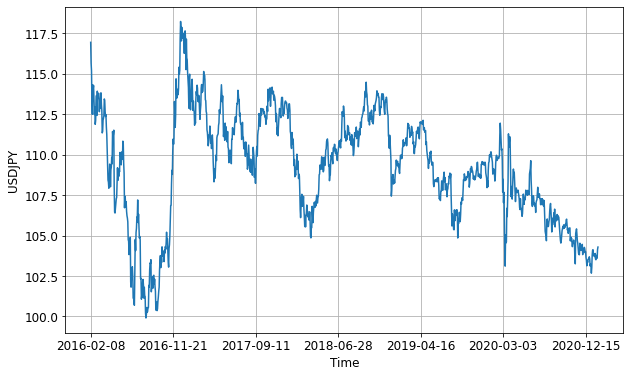
\includegraphics[width=10cm]{hw1_yt.png}
    \caption{Display of Y(t) over Time}
    \label{yt}
\end{figure}

\begin{figure}[h]
    \centering
    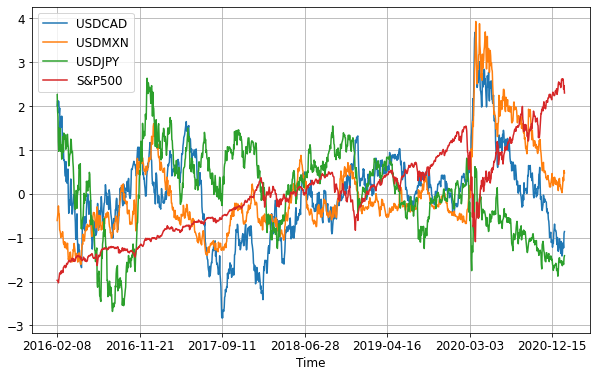
\includegraphics[width=10cm]{hw1_allseries.png}
    \caption{Normalized Display of All Indices}
    \label{allseries}
\end{figure}

\begin{figure}[h]
    \centering
    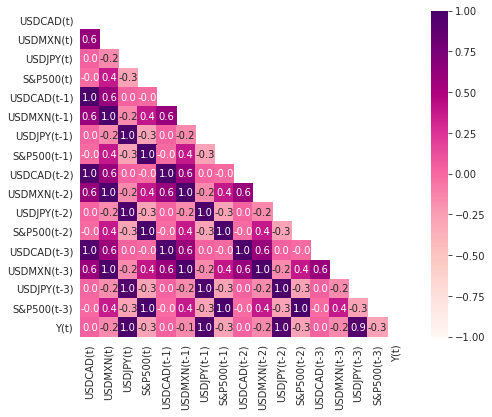
\includegraphics[width=13cm]{hw1_corr.png}
    \caption{Correlation Matrix}
    \label{corr}
\end{figure}

\newpage

\question*{Structure of the MLP}
A MLP is a dense artificial neural network, where each neuron is connected to every neuron in the previous layer and every neuron in the subsequent layer. for our MLP, three layers were used. These consits of an input layer, a hidden layer, and an output layer. The input layer has dimension 16; it is the input vector V(t) mentioned in Section 1. It containins all features save JPY(t+1). The output layer has dimension 1. It contains a single neuron with the predicted price of the yen, MLP[JPY(t+1)].\\\\
The dimension of the hidden layer, h, is selected by repeated trials. It is typically chosen so the number of neurons minimizes the mean squared error (MSE) of the output. The selection of h is  explored further in Section 3.\\\\
The layers of the MLP are "connected" by weights, which represent each neuron's effect on the other neurons. The input layer has 16 neurons, one for each of the features. Thus, 16*h weights connect the input layer to the hidden layer. Since the output layer contains single neuron, there are h weights connecting the hidden layer to the output layer. Each connection also contains a threshold, a parameter which acts like the intercept term in a simple linear regression. A total of h thresholds connect the input layer to the hidden layer and h additional thresholds connect the hidden layer to the output layer. There is an additional threshold on the output layer. This results in a total number of parameters (weights and thresholds) of 18h+1.\\\\
Each neuron updates its state depending on these weights and thresholds, as well an activation function which is selected prior to network construction. We have chosen the RELU activation function which takes the maximum between the function's input and 0. This results in efficient computation and strictly non-negative values. As predicting negative prices are inappropriate for this domain, this response function is both sensible and efficient.\\\\
Together, the jth neuron's state is represented as follows:
\begin{center} \begin{math}
f(x_j) = max(0, w_0 + \sum_{j=1}^{J} w_j*x_{j-1}) 
\end{math} \end{center}
where w$_0$ is the threshold, w$_j$ is the column of weights corresponding to neuron j, and x$_{j-1}$ is neurons of the previous layer.

\question*{Choosing H}
We now go about selecting the best value for h. We randomly split our 1231 cases into training and testing sets. For an 80-20 split, this gives a training set size of 985 and a test set size of 246. We next place a constraint on h, to increase the generalizing ability of our MLP. We want 18h+1 to be lower than the number of cases in our training set. With a training set size of 985, this gives us \textbf{a maximum value of 54 for h}.
\\\\
We then centered and re-scaled our input vector by each feature's means and standard deviations, and performed Principal Components Analysis (PCA) to reach an explained variance of 95\%. Curves of the eigenvalues and percentage of variance explained are displayed in Figure \ref{pca}. Four principal components are required to reach this percentage and this becomes our \textbf{minimum value of h, 4}. To fill out this range we selected \textbf{two more potential values of h}, choosing the approximately equidistant values \textbf{21 and 37}.\\\\

\begin{figure}[h]
\begin{subfigure}{0.45\textwidth}
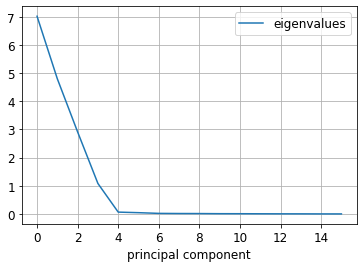
\includegraphics[width=\linewidth]{h1_pca_eigen.png}
\caption{Eigenvalues}
\end{subfigure}
\hfill % max horizontal distance between graphs
\begin{subfigure}{0.45\textwidth}
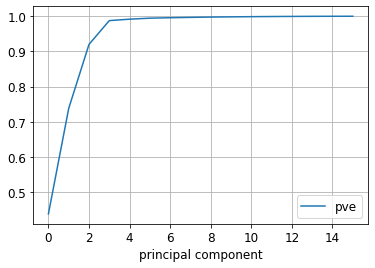
\includegraphics[width=\linewidth]{h1_pca_pve.png}
\caption{Percentage of Variance Explained}
\end{subfigure}
\caption{Principal Components Analysis}
\label{pca}
\end{figure}

The implementation of automatic learning was accomplished using tensorflow on Google Colab's IDE. The learning utilized ADAM gradient descent, batch learning with a batch size of 25, and the loss-function taken to be the minimization of the MSE. We also  considered the Average Relative Error (AvRelErr), defined as \begin{math} AvRelErr = \frac{1}{N}\sum_{i=1}^{N} \frac{|y^`_i - y_i|}{y_i} \end{math}, where y$^`$ $_i$ is the predicted value for JPY(t+1) and y$_i$ is the true value. Additionally, Rescaled RMSE was considered, which is \begin{math} RescRMSE = \frac{\sqrt{MSE}}{avg(Y(t))} \end{math}. Ideally, we will choose the h which contains the minimum value for all the metrics. The results for our potential h values are displayed in Table \ref{h_select}.

\begin{table}[H]
    \centering
    \begin{tabular}{c|cccc}
         h&Best Train MSE&Best Test MSE&AvRelErr&RescRMSE\\\hline
         4&1.59&2.87&0.010&0.016 \\
         21&0.56&0.71&0.006&0.008\\
         37&0.72&1.00&0.007&0.009\\
         54&0.82&1.19&0.007&0.010
    \end{tabular}
    \caption{Four Potential Values of h}
    \label{h_select}
\end{table}

Additionally, plots of the MSE and gradient(||MSE||) for each h value are shown in Figure \ref{batch_evo}. At h = 4 the gradient(||MSE||) does not begin to stabilize until around the 2000th batch, near where MSE reaches its minimum value. For the other h-values the gradient stabilizes much earlier, at around batch 500. Likewise, MSE reaches its minimum value much quicker, indicating that our hidden layer needs to be larger than the 4 principal components. \newpage  

\begin{figure}[H]
\begin{subfigure}{0.4\textwidth}
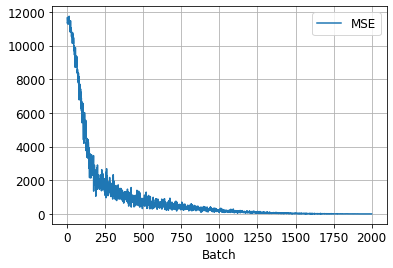
\includegraphics[width=\linewidth]{h4_MSE.png}
\caption{h=4, MSE} \label{fig:a}
\end{subfigure}\hspace*{\fill}
\begin{subfigure}{0.4\textwidth}
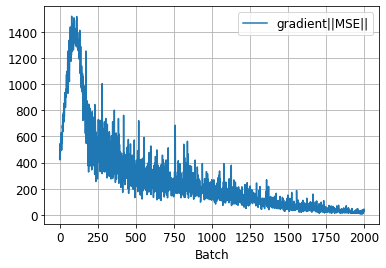
\includegraphics[width=\linewidth]{h4_gradient.png}
\caption{h=4, grad(||MSE||)} \label{fig:b}
\end{subfigure}

\medskip
\begin{subfigure}{0.4\textwidth}
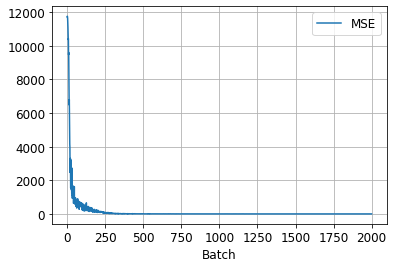
\includegraphics[width=\linewidth]{h21_MSE.png}
\caption{h=21, MSE} \label{fig:c}
\end{subfigure}\hspace*{\fill}
\begin{subfigure}{0.4\textwidth}
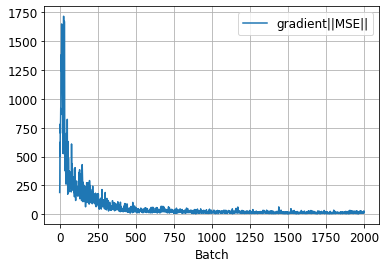
\includegraphics[width=\linewidth]{h21_gradient.png}
\caption{h=21, grad(||MSE||)} \label{fig:d}
\end{subfigure}

\medskip
\begin{subfigure}{0.4\textwidth}
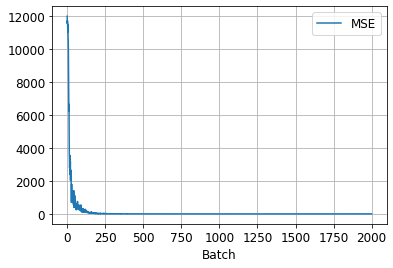
\includegraphics[width=\linewidth]{h37_MSE.png}
\caption{h=37, MSE} \label{fig:e}
\end{subfigure}\hspace*{\fill}
\begin{subfigure}{0.4\textwidth}
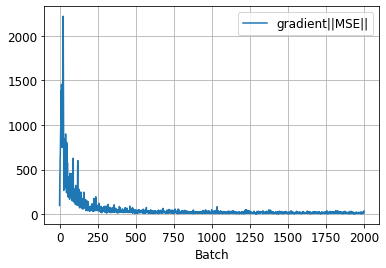
\includegraphics[width=\linewidth]{h37_gradient.png}
\caption{h=37, grad(||MSE||)} \label{fig:f}
\end{subfigure}

\medskip
\begin{subfigure}{0.4\textwidth}
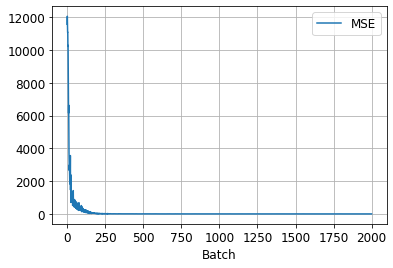
\includegraphics[width=\linewidth]{h54_MSE.png}
\caption{h=54, MSE} \label{fig:g}
\end{subfigure}\hspace*{\fill}
\begin{subfigure}{0.4\textwidth}
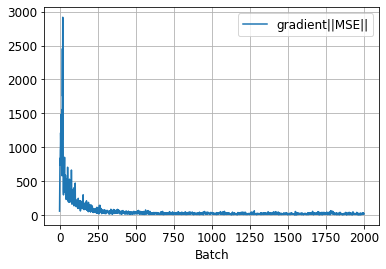
\includegraphics[width=\linewidth]{h54_gradient.png}
\caption{h=54, grad(||MSE||)} \label{fig:h}
\end{subfigure}

\caption{Plots of MSE and grad(||MSE||) for each h Value} \label{batch_evo}
\end{figure} \newpage

To further select from between the remaining values of h, we plotted the performance on the training and testing sets as in Figure \ref{train_test}. The test MSE for h=4 is very large, and it doesn't reach its minimum value, 2.87, until very late in the learning. At h=21, the test MSE decreases at a consistent rate, eventually stabilizing around the 35th epoch before settling at its lowest value, 0.71. At h=37, the test MSE likewise stabilizes around the 35th epoch, then reaching its minimum value of 1.00. H=54's learning is more erratic, but it begins to stabilize at epoch 30, before randomly fluctuating around 1.5 for 15 epochs, and then decreasing sharply to its minimum value of 1.19.\\\\
While these graphs do not provide clear direction for the best value of h, Table \ref{h_select} does. \textbf{H=21} has the lowest test MSE, the lowest Average Relative Error, and the lowest Rescaled RMSE. It is our best value for h. A plot of its predicted values for Y(t) and the actual values of Y(t) are displayed in Figure \ref{pred_v_actual}. For the most part, it tracks the series very well, with consistently larger errors coming in the small window between 1000 and 1075 t.

\begin{figure*}
\begin{subfigure}{0.45\textwidth}
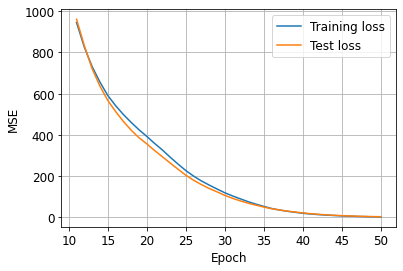
\includegraphics[width=\linewidth]{h4_loss.png}
\caption{h=4}
\end{subfigure}
\hfill % max horizontal distance between graphs
\begin{subfigure}{0.45\textwidth}
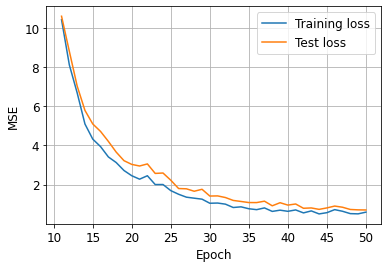
\includegraphics[width=\linewidth]{h21_loss.png}
\caption{h=21}
\end{subfigure}

\medskip
\begin{subfigure}{0.45\textwidth}
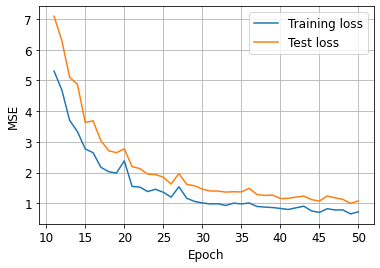
\includegraphics[width=\linewidth]{h37_loss.png}
\caption{h=37}
\end{subfigure}
\hfill 
\begin{subfigure}{0.45\textwidth}
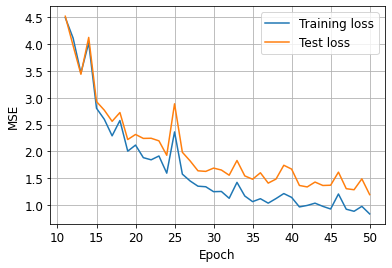
\includegraphics[width=\linewidth]{h54_loss.png}
\caption{h=54}
\end{subfigure}

\caption{MSE Plots for different h Values on the Training and Testing Set} \label{train_test}
\end{figure*}

\begin{figure}[h]
    \centering
    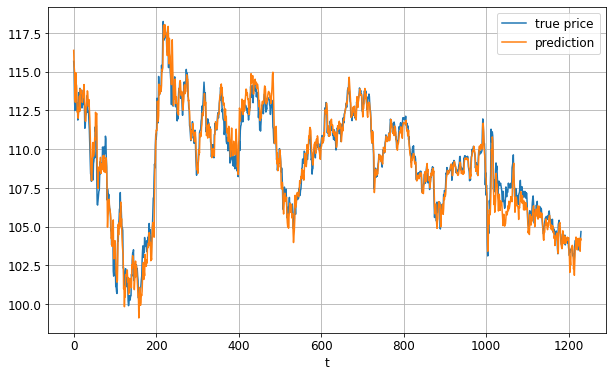
\includegraphics[width=10cm]{hw1_predvactual.png}
    \caption{MLP's Predicted Value of Y(t) and Actual Value of Y(t)}
    \label{pred_v_actual}
\end{figure}

\question*{Neuron Activity}
With our best h-value of 21, our MLP is now fixed. It has 16 input neurons, a hidden layer with 21 neurons, and a single output neuron. Its weights and thresholds have been determined by automatic learning to minimize MSE. We are now interested in the activity levels of these 21 neurons. Active neurons are those which have a large effect on the predicted value of Y(t), MLP[JPY(t+1)]. Neurons which have a very small effect on this prediction may be inessential to the learning. By identifying these neurons, we may be able to prune them, thus making our MLP faster and more efficient.\\\\
A plot of the average activity of the neurons is displayed in Figure \ref{neurons}. The most active neuron has an average activity level of close to 5, while the least active neuron (displayed at x=0) has an average activity of about 1. Fifteen of the neurons have an average activity between 3.5 and 4.5, indicating that most of the neurons in the hidden layer are participating equally in the work of predicting JPY(t+1). 

\begin{figure}[H]
    \centering
    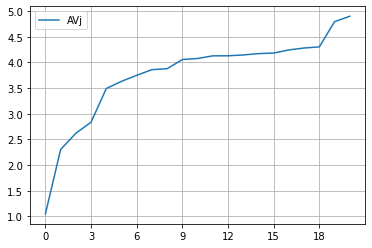
\includegraphics[width=8cm]{h21_neurons.png}
    \caption{Average Activity of Neurons for Best MLP}
    \label{neurons}
\end{figure}

\begin{table}[H]
    \centering
    \subfloat[Most Active Neurons]{\begin{tabular}{c|c}
         Neuron&Activity Level\\\hline
         16&4.90 \\
         17&4.79\\
         12&4.30
    \end{tabular}}\\
    \subfloat[Least Active Neurons]{\begin{tabular}{c|c}
         Neuron&Activity Level\\\hline
         20&1.05 \\
         11&2.30\\
         8&2.62
    \end{tabular}}
    \caption{Most and Least Active Neurons}
    \label{neurons}
\end{table}

Further examining the most and least active neurons may be instructive, as the magnitude of their respective weights may provide us with additional insight regarding the MLP's goal. From Table \ref{neurons} we know the most active neuron, Neuron 16, has an average activity of about five, while the least active neuron has an average activity of about 1.\\\\
Table \ref{most_active} shows the weights connecting the input layer to the most active neuron along with the corresponding features. All time delays for S&P 500 have the greatest affect in predicting JPY(t+1), followed by all time delays for JPY. The presence of JPY among the most important features is not surprising, however, the outsized effect of S&P 500 is. It is the most important feature for the most active neuron. Alternatively, the CAD and MXN are not very important for the most active neuron.
The least active neuron's weights and features are displayed in Table \ref{least_active}. In an about-face from the most active neuron, the least active neuron is most influenced by CAD and MXN, and least influenced by S&P 500 and JPY.

\begin{table}[H]
    \centering
    \begin{tabular}{c|c}
         Feature&Weight \\\hline
         SP(t)&1.350 \\
         SP(t-1)&1.349\\
         SP(t-2)&1.229\\
         SP(t-3)&1.198\\
         JPY(t-3)&0.744\\
         JPY(t)&0.621\\
         JPY(t-1)&0.516\\
         JPY(t-2)&0.429\\
         CAD(t-1)&0.210\\
         MXN(t-2)&0.183\\
         CAD(t-3)&0.182\\
         CAD(t)&0.114\\
         MXN(t)&-0.309\\
         MXN(t-3)&-0.346\\
         MXN(t-1)&-0.435\\
         CAD(t-2)&-0.476
    \end{tabular}
    \caption{Most Active Neuron's Features and Weights}
    \label{most_active}
\end{table}

\begin{table}[H]
    \centering
    \begin{tabular}{c|c}
         Feature&Weight \\\hline
        CAD(t-1)&0.499\\
        MXN(t-2)&0.490\\
        CAD(t-3)&0.332\\
        MXN(t-3)&0.176\\
        MXN(t)&0.099\\
        MXN(t-1)&0.062\\
        CAD(t-2)&-0.079\\
        CAD(t)&-0.230\\
        JPY(t-3)&-0.488\\
        JPY(t-1)&-0.671\\
        JPY(t-2)&-0.834\\
        JPY(t)&-1.028\\
        SP(t)&-1.214\\
        SP(t-2)&-1.239\\
        SP(t-1)&-1.301\\
        SP(t-3)&-1.358
    \end{tabular}
    \caption{Least Active Neuron's Features and Weights}
    \label{least_active}
\end{table} 

\question*{Removing the Least Active Neuron}
We decided to remove the least active neuron from the MLP, interested in what would happen if Neuron 20, with an activity level less than half of the next least active neuron, was no longer part of the network. This process entailed setting all the weights connecting Neuron 20 to the rest of the MLP to 0.\\\\
The 'new' MLP has a Rescaled RMSE of 0.010 and an Average Relative Error of 0.007, placing it in the same territory as MLPs for h=37 and h=54. It is likely that Neuron 20's activity, while relatively low at an average value of 1, was not low enough to warrant elimination from the network.

\question*{Conclusion and Final Thoughts}
While homework is not normally assigned to help students make "Jim Cramer shouting with glee on CNBC" money, we hoped this MLP would be an accidental moneymaker, allowing us to go to class, trade some Yen, and rest on our golden laurels.\\\\
Our best MLP had an average relative error of 0.006, meaning that its prediction for JPY(t+1) missed the true value by about 0.6\%. While this is a decent performance, 0.6\% can be the difference between making and losing money, depending on the fluctuations in the forex market.\\\\
As a result, we've decided, at least for the moment, to refrain from trading forex like madmen.
\newpage
\lstinputlisting{code.py}
\end{document}
